\documentclass[twoside]{ausarbeitung}

%\usepackage{apacite}
\usepackage[notocbib]{apacite}
%\usepackage{endfloat}

% ----------------------------------------------

\begin{document}

\selectlanguage{english}

\author{Beytullah Ince}
\title{\textbf{Reinforcement Learning for Strategy Games}}
\doctype{Thesis}

\examinerA{Prof.~Dr.~Ulrich~Klauck}
\examinerB{Prof.~Dr.~Martin~Heckmann}
\date{Januar 2022}

\maketitle
\cleardoublepage

\pagenumbering{Roman}
\setcounter{page}{1}

\tableofcontents

\addcontentsline{toc}{chapter}{List of Figures}
\listoffigures

\addcontentsline{toc}{chapter}{List of Tables}
\listoftables

\cleardoublepage
\pagenumbering{arabic}
\setcounter{page}{1}


% ------------------------------------------------------------------------------------------------------------------------------------------------------------------------------------------------------------
% ------------------------------------------------------------------------------------------------------------------------------------------------------------------------------------------------------------

\chapter{Introduction}
Sudoku is a single player puzzle game. The game is played on a grid, which consists of 9x9 cells. Numbers ranging from 1 to 9 must be filled into all cells without violating the rules. Based on the difficulty of the puzzle, varying count of numbers are given at the start of the game. The grid can be separated into rows, columns and into blocks, which consists of 3x3 cells. In none of the rows, columns, or blocks is it allowed to repeat the same number. These are the rules, that will be used throughout this paper. There are also other variations of the game, but those will not be discussed.
The goal of this paper is to present various techniques to solve the sudoku puzzle.

% ------------------------------------------------------------------------------------------------------------------------------------------------------------------------------------------------------------
% ------------------------------------------------------------------------------------------------------------------------------------------------------------------------------------------------------------

\chapter{Kapitel A}


\blindtext

\section{Erster Abschnitt}

\par\blindtext
\par\blindtext

\section{Zweiter Abschnitt}

\par\blindtext
\par\blindtext
\par\blindtext
\par\blindtext
\par\blindtext

% ------------------------------------------------------------------------------------------------------------------------------------------------------------------------------------------------------------
% ------------------------------------------------------------------------------------------------------------------------------------------------------------------------------------------------------------

\chapter{Kapitel B}

\par\blindtext
\par\blindtext

\section{Erster Abschnitt}

\par\blindtext
\par\blindtext

\section{Zweiter Abschnitt}

\par\blindtext
\par\blindtext
\par\blindtext

% ------------------------------------------------------------------------------------------------------------------------------------------------------------------------------------------------------------
% ------------------------------------------------------------------------------------------------------------------------------------------------------------------------------------------------------------




% ------------------------------------------------------------------------------------------------------------------------------------------------------------------------------------------------------------
% ------------------------------------------------------------------------------------------------------------------------------------------------------------------------------------------------------------




% ------------------------------------------------------------------------------------------------------------------------------------------------------------------------------------------------------------
% ------------------------------------------------------------------------------------------------------------------------------------------------------------------------------------------------------------
















































\chapter{Techniques}

There are various techniques to solve sudoku puzzles. Some of the techniques are easy to spot and use, while others are harder. 
In this chapter several techniques are explained. The selection is based on how often the techniques appeared during the research and will be categorized into different level of difficulties.


\section{Basics}
\subsection{Candidates and Pencil Marks}
Candidate is a term used to describe possible values or digits. Usually, cells are occupied by a digit or are empty. By using different techniques, it is possible to narrow down the possible values for cells. Those values are written down in a much smaller size, as seen in Figure \ref{fig:pmarks} and are referred as pencil marks \cite{Diagrams86:online}.

\begin{figure}[H]
  \centering
  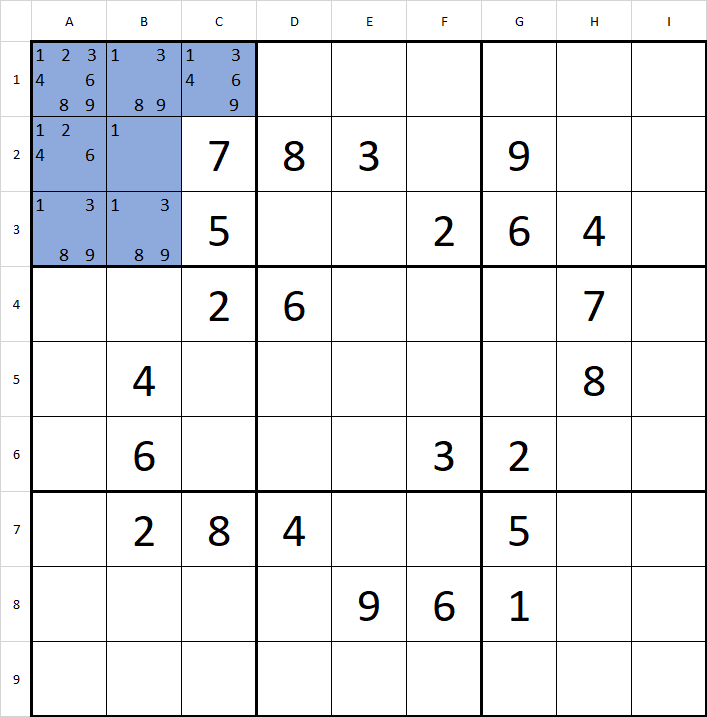
\includegraphics[width=.475\linewidth]{images/pmarks.png}
  \caption[Pencil Marks]{Pencil Marks indicated by blue background. Source: Adapted from \cite{SolvingS57:online}}
  \label{fig:pmarks}
\end{figure}%

With pencil marks, the player does not have to memorize all candidates. Furthermore, the player can use techniques to eliminate candidates from cells, to narrow down the real value.

\subsection{Cross-Hatching} \label{ss:xhatching}
In Cross-Hatching the player is looking for a digit which has already been placed and draws imaginary lines from that digit its cell across rows and column \cite{HowtoSol27:online}. This way the player can identify in which cells, the digit cannot be placed into and in which it can, as demonstrated in Figure \ref{fig:xhatching}.

\begin{figure}[H]
  \centering
  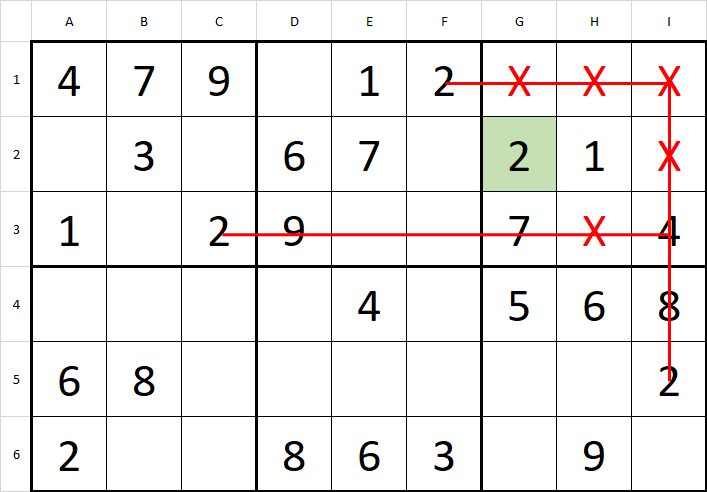
\includegraphics[width=.5\linewidth]{images/xhatching}
  \caption[Cross-Hatching] By Cross-Hatching the two from C3, F3 and I5 it was possible to narrow down the cell for the two in the 3$^{rd}$ block. The red lines are indicating the imaginary lines, the red cross indicates the cells, which cannot have a two and the green backgrounded cell highlights the only cell, which can have a two.
  \label{fig:xhatching}
\end{figure}%

For the case that enough digits are placed, the player can directly place the digit which was used for the Cross-Hatching. Alternatively, it is possible to use pencil marks, to narrow down the candidates by removing that digit.

\subsection{Snyder Notation} \label{ss:snydernot}
The Snyder Notation is a technique for pencil marking candidates. However, instead of pencil marking all possible candidates, the pencil marks are only done for candidates that can be limited to two cells in a block \cite{ExpertSu16:online}. 

\begin{figure}[H]
  \centering
  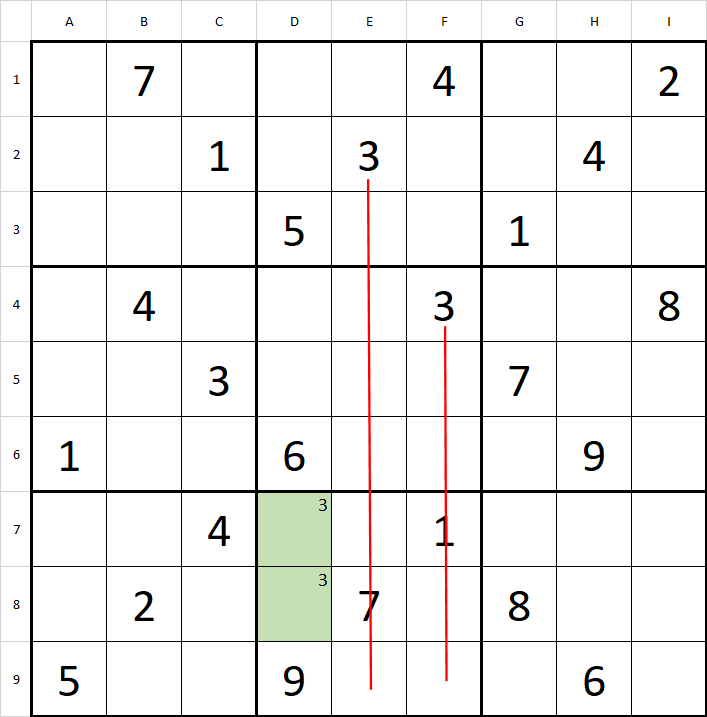
\includegraphics[width=.5\linewidth]{images/snyder}
  \caption[Snyder Notation]Snyder Notation. The 3's in E2 and F4 eliminates all candidates but two, in block 8. The cells with the Snyder Notation are highlighted by green background. In this example \nameref{ss:xhatching} was used to apply the technique. Source: Adapted from \cite{ExpertSu16:online}
  \label{fig:snyder}
\end{figure}%

The beneift of this technique is that as soon as one of the cells is filled, the other ones trie value is automatically the candidates, since those were the only two cells for the candidate.


\section{Easy}

\subsection{Full House}
The Full House can be used when a group (row, column, or a block) has been entirely filled out, except a single cell. The cell its value is the missing one from the range one to nine and can be filled into the empty cell \cite{SolvingS57:online}.  


\subsection{Naked Single}
The Naked Single requires the usage of pencil marks to determine the candidates for cells. If a cell has only one candidate left then it is a Naked Single \cite{SudokuLo64:online}.

\subsection{Hidden Single}
A Hidden Single is like a Naked Single. The technique also requires the usage of candidates and finding a sole candidate. However, for this technique it is required that the candidate is the only one of its kind within a group and hidden among other candidates in its cell \cite{SolvingS57:online}, as shown in  Figure \ref{fig:hiddensingle}.

\begin{figure}[H]
  \centering
  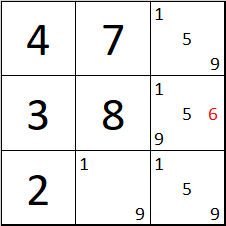
\includegraphics[width=.25\linewidth]{images/hiddensingle}
  \caption[Hidden Single] A hidden single inside of a block indicated by red color. The six does not appear in any other of the cells as a candidate, therefore it must go into that cell. Source: Adapted from \cite{SolvingS57:online}
  \label{fig:hiddensingle}
\end{figure}%

The reason for this is, that all digits from one to nine have to appear in a group and since the other cells do not have that candidate, there is only one cell it can be placed in.

\subsection{Naked Pair} \label{ss:npair}
Naked pairs are pairs of identical candidates within a group. The candidates of a naked pair can be removed from the possible candidates of all cells in the group, as seen in Figure \ref{fig:nakedpair}. 

\begin{figure}[H]
  \centering
  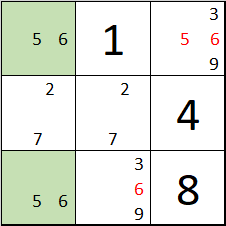
\includegraphics[width=.25\linewidth]{images/nakedpair}
  \caption[Naked Pair] A naked pair highlighted by green background. The red colored digits are the eliminated possible candidates, due to the pair. Source: Adapted from \cite{NakedPai2:online}
  \label{fig:nakedpair}
\end{figure}%

The reason for this is that the digits of the candidate pair can only be contained from that cells \cite{NakedPai2:online}.

This technique can be extended to Naked Triple and Naked Quad. Both behave the same, but with more identical candidates. The difficulty of these techniques is higher because they are harder to spot.













\section{Medium}

\subsection{Hidden Pair} \label{ss:hpair}
A hidden pair is like a \nameref{ss:npair}, but it is hidden among other candidates, therefore, it is harder to spot and more difficult. Figure \ref{fig:hiddenpair} shows a hidden pair and compared to the \nameref{ss:npair}, the cells contain other pencil marks \cite{SudokuHi85:online}.

\begin{figure}[H]
  \centering
  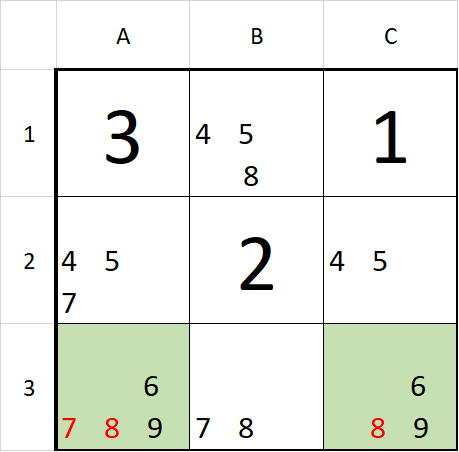
\includegraphics[width=.25\linewidth]{images/hiddenpair}
  \caption[Hidden Pair] The cell with a hidden pair is highlighted by green background. The red colored digits are the eliminated possible candidates, due to the pair. Source: Adapted from \cite{SudokuHi85:online}
  \label{fig:hiddenpair}
\end{figure}%

This technique is also extendable, which are named Hidden Triple and Hidden Quad. The difficulty to spot these techniques is also higher than spotting Hidden Pairs.

\subsection{Locked Candidates} \label{ss:lcandidates}
There are two variations of the Locked Candidates. One is applied to a row, or column and the other one to a block. The requirements for the first variation is that in one of three blocks, a candidate must be restricted to one row or column, as seen in Figure \ref{fig:lcandidate1}. By doing that, the candidate is eliminated in the other blocks for the same row, or column, because the candidate can only appear once in a row, or column. 

\begin{figure}[H]
\centering
\begin{subfigure}[t]{.625\textwidth}
  \centering
  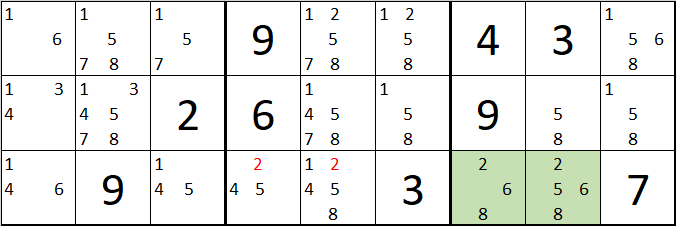
\includegraphics[width=\linewidth]{images/lcandidate1}
  \caption{Variation one eliminates candidates in the same row, or column. Source: Adapted from: \cite{SolvingS57:online}}
  \label{fig:lcandidate1}
\end{subfigure}%
\hfill
\begin{subfigure}[t]{.325\textwidth}
  \centering
  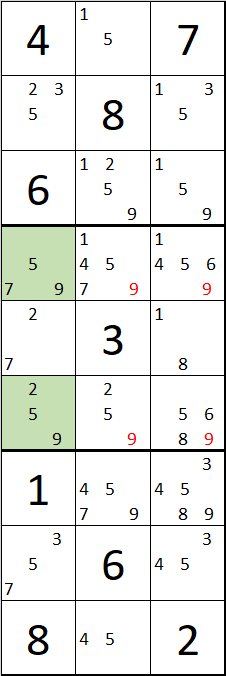
\includegraphics[scale=.50]{images/lcandidate2}
  \caption{Variation two eliminates candidates in the same block. Source: Adapted from: \cite{SolvingS57:online}}
  \label{fig:lcandidate2}
\end{subfigure}
\caption[Locked Candidates]{Locked Candidates variation 1 and 2. Candidates who met the requirements are highlighted with green background and the eliminated candidates with red color.}
\label{fig:lcandidate}
\end{figure}


In the second variation a candidate can be eliminated from the remaining cells of a block, when it is the only one appearing across  a row, or column \cite{SolvingS57:online}, as shown in Figure \ref{fig:lcandidate2}.


\subsection{Skyscraper} \label{ss:sky}
The requirement for the Skyscraper technique is to find two rows, or columns, which have exactly two candidates and one identical candidate. Additionally, the identical candidate must be in the same column, or row, as illustrated in Figure \ref{fig:skyscraper}.

\begin{figure}[H]
  \centering
  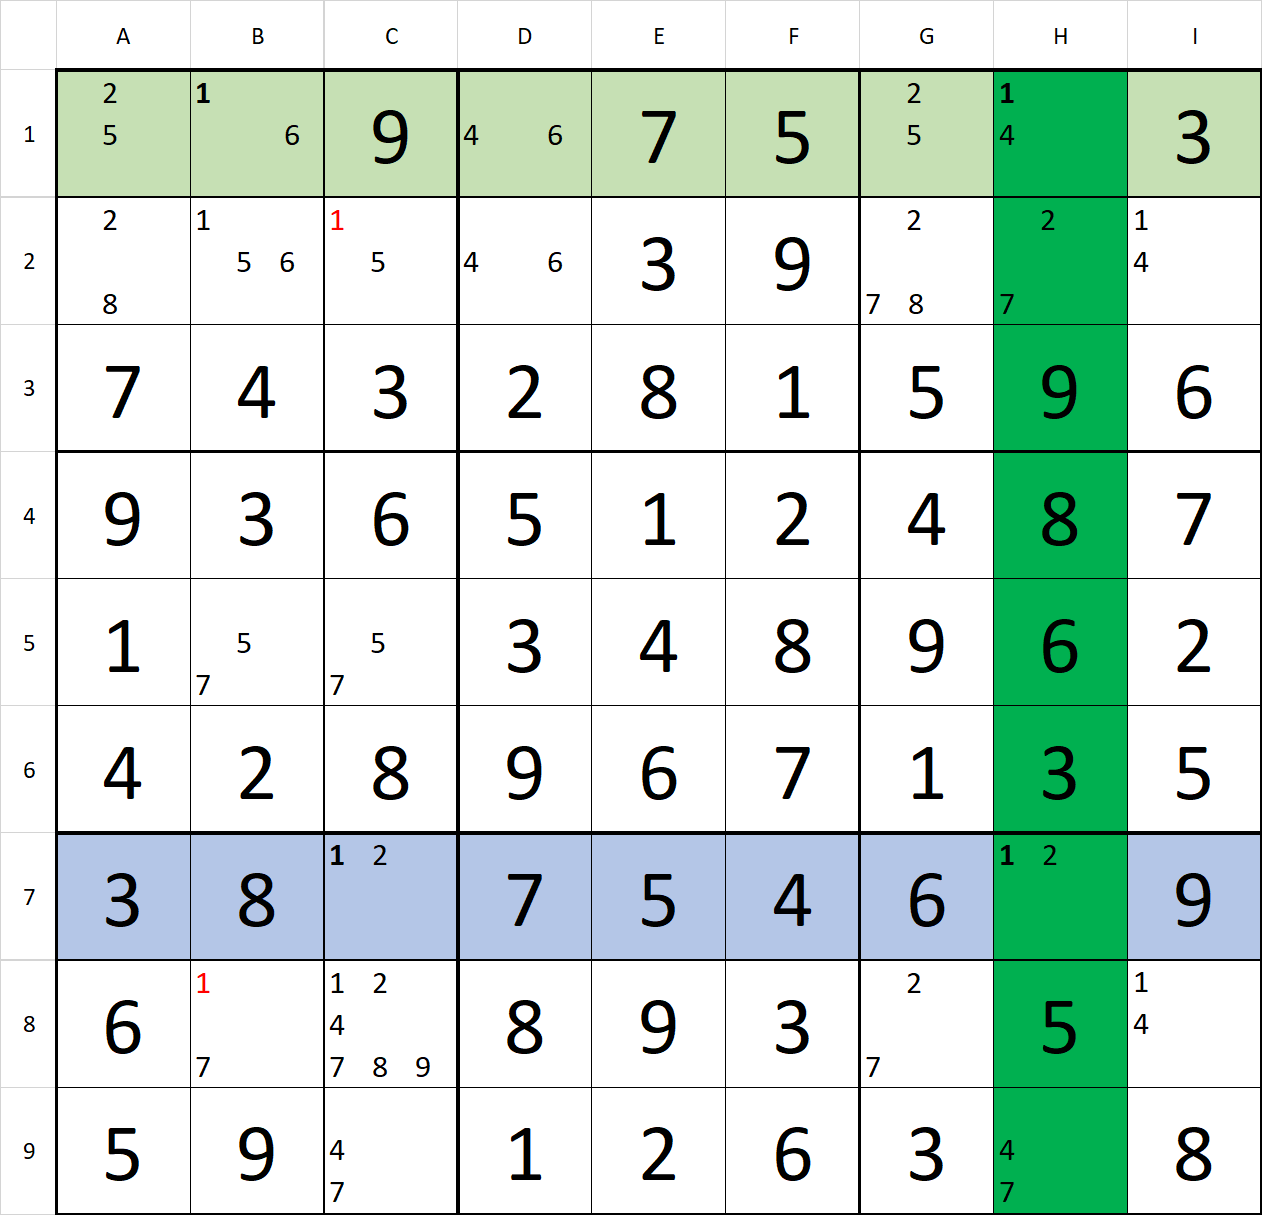
\includegraphics[width=.55\linewidth]{images/skyscraper}
  \caption[Skyscraper] Skyscraper Technique. One is the digit that appears only twice in two rows and is one of the naked pairs' digit. It is highlighted by light green and light blue background. The green background indicates the column in which the digit appears twice (H1 and H7). Digits with red color indicate the eliminated candidates. Source: Adapted from \cite{SudokuSk81:online}
  \label{fig:skyscraper}
\end{figure}%

With this setup, the candidate must be placed in one of the opposing candidate cells, because of the identical candidate in the same column, or row. Therefore, the candidate for the digit can be eliminated from the respective column, or row.
\cite{SudokuSk81:online}


\subsection{2-String Kite}

The 2-String Kite technique is similar to the \nameref{ss:sky} technique. It is required to find two cells with exactly two candidates and one identical one. It is required to find two cells in the same block, that are the only ones with an identical candidate. One of these cells must have another cell in the row, which is the only one that has the identical candidate. Likewise, the other cell in regards of a column \cite{Sudoku2S39:online}. Thus, the identical candidate at the intersection of these extra cells, can be eliminated, which is illustrated in Figure \ref{fig:2skite}.

\begin{figure}[H]
  \centering
  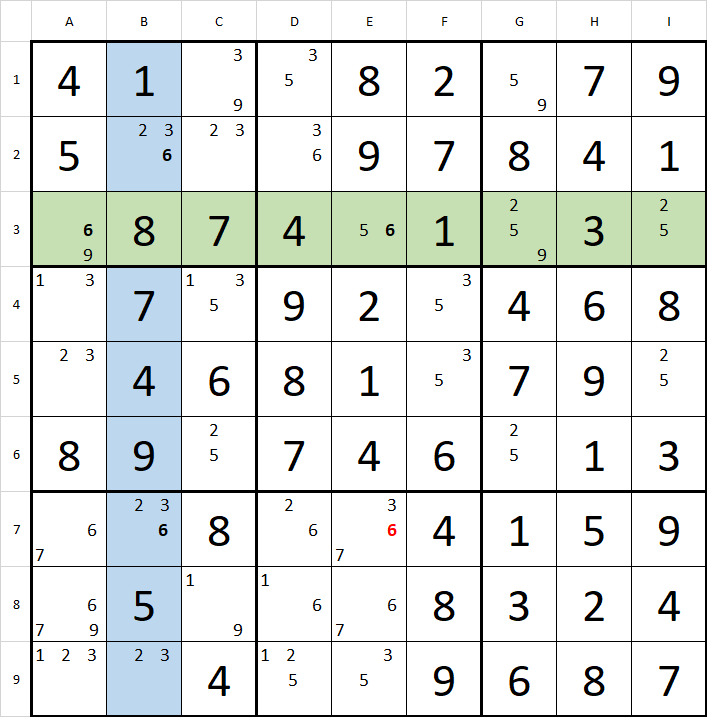
\includegraphics[width=.55\linewidth]{images/2skite}
  \caption[2-String Kite] 2-String Kite Technique. A3 and B2 share an identical candidate in the same block. B2 shares the candidate with B7 in the same column and A3 with E3 in the same row. The candidate appears only twice in both, the column and row, which are highlighted by blue and green background color, respectively. The eliminated in E7 is highlighted by red color, which is the intersection between the extra cells. Source: Adapted from \cite{AHRSudok73:online}
  \label{fig:2skite}
\end{figure}%











\section{Hard}

\subsection{X-Chain} \label{ss:xchain}
Only one candidate is taken into consideration for the X-Chain technique. The cells for this technique must be linked in a specific way. For the first and last cell of the chain, the number of cells that the candidate can go within their respective group, is limited to two. For the other cells it is necessary to be in a group. This ensures that the candidate can be eliminated from cells who shares a group with the first and last cell of the chain \cite{XChainSu93:online}, as illustrated in Figure \ref{fig:xchain}.

\begin{figure}[H]
  \centering
  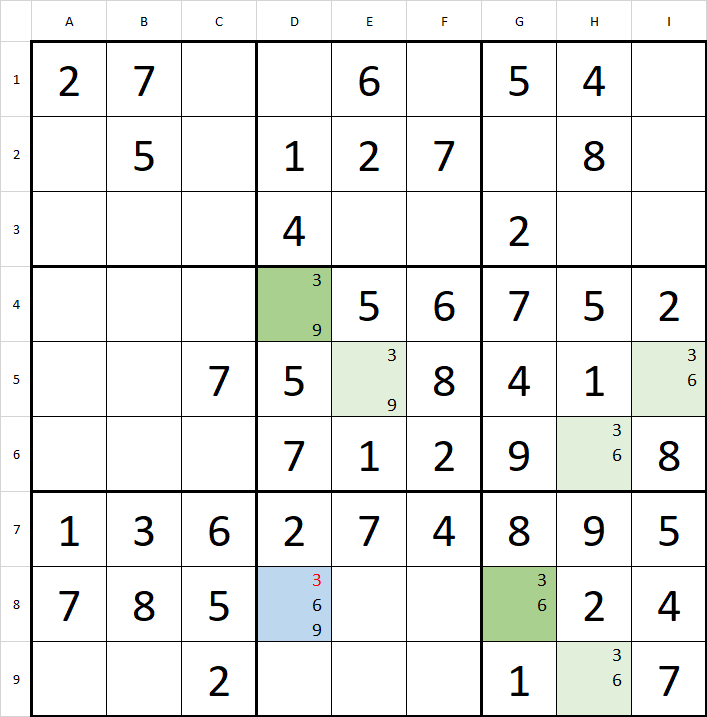
\includegraphics[width=.55\linewidth]{images/xchain}
  \caption[X-Chain] X-Chain Technique. The candidate in this case is 3. First and last cell (D4, G8) are highlighted by green background, the other cells by light green background. Source: Adapted from \cite{XChainSu93:online}
  \label{fig:xchain}
\end{figure}%

The connection between the cells ensures, that the chosen candidate can only go into the first, or last cell. Therefore, the candidate can be eliminated from the cells, that share a group with them.

\subsection{XY-Chain}
The XY-Chain is similar to the \nameref{ss:xchain}. The difference is that in the XY-Chain technique that all the cells can only have two candidates. The illustration in Figure \ref{fig:xychain} shows, that the result is the same. The candidate in all cells that are in a group with the first and last cell, can be eliminated \cite{SudokuXY13:online}.


\begin{figure}[H]
  \centering
  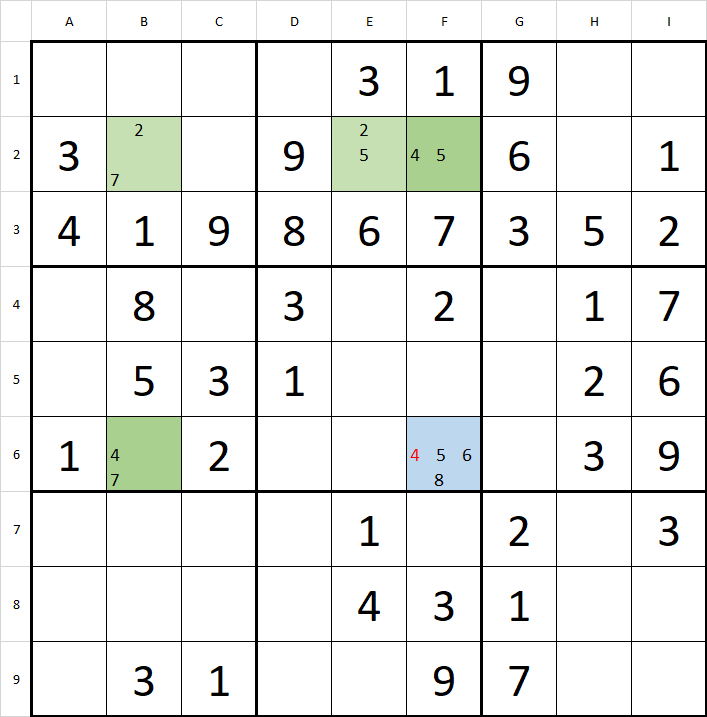
\includegraphics[width=.55\linewidth]{images/xychain}
  \caption[XY-Chain] XY-Chain Technique. The candidate in this example is 4. The first and last cell are highlighted by green background (F2, D8). The cells that link them together are highlighted with light green background. Blue background color indicates the cells, on which the technique is applied. The removed candidate is indicated by red color.  Source: Adapted from \cite{SudokuXY13:online}
  \label{fig:xychain}
\end{figure}%


\subsection{W-Wing}
The W-Wing technique requires a chain between four cells. The first and last cell (main cells) must share their only two candidates. The other two cells (branch cells) must share one of the two candidates. Furthermore, each main cell must be aligned in a row, or column with one of the branch cells. Additionally, the candidate for the branch cells must be the only one of its kind in their group. If these requirements are met, then the other candidate can be removed from all cells, that share a group with the main cells \cite{WWingSud29:online}, as demonstrated in Figure \ref{fig:wwing}.

\begin{figure}[H]
  \centering
  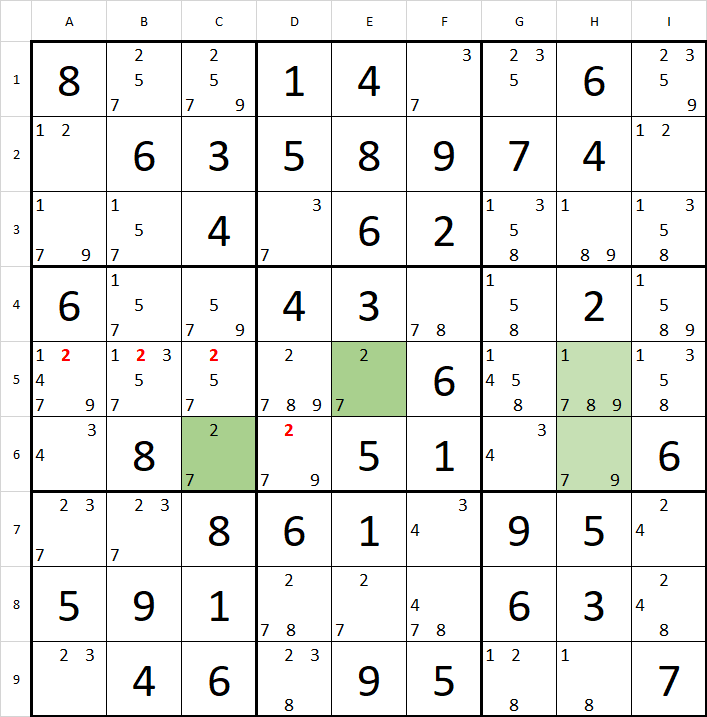
\includegraphics[width=.55\linewidth]{images/wwing}
  \caption[W-Wing] W-Wing Technique. The main cells are highlighted by green background and the branch cells with a light green background. The candidate that is eliminated has red color. The main cells share the candidates 2 and 7. Both main cells are a row with a two cells, that are the only candidates for 7 in their respective group. Therefore, the other candidate (2) can be eliminated from all cells that share a group with the main cells (A5, B5, C5 and D6). Source: Adapted from \cite{WWingSud29:online}
  \label{fig:wwing}
\end{figure}%

The logic behind this technique is that if one of the branch cells takes the candidates value, then the main cell in the same row must take the value of the other candidate, leading to the elimination of that candidate in shared groups, vice versa for the other branch cells. Since the cells are chained with each other, the candidate gets eliminated in both scenarios.


\subsection{X-Wing} \label{sec:xwing}
The X-Wing technique requires four candidates of the same digit. The candidates must be aligned in either two parallel columns or two parallel rows on the same cells, as depicted in Figure \ref{fig:xwing}. 

\begin{figure}[H]
\centering
\begin{subfigure}[t]{.475\textwidth}
  \centering
  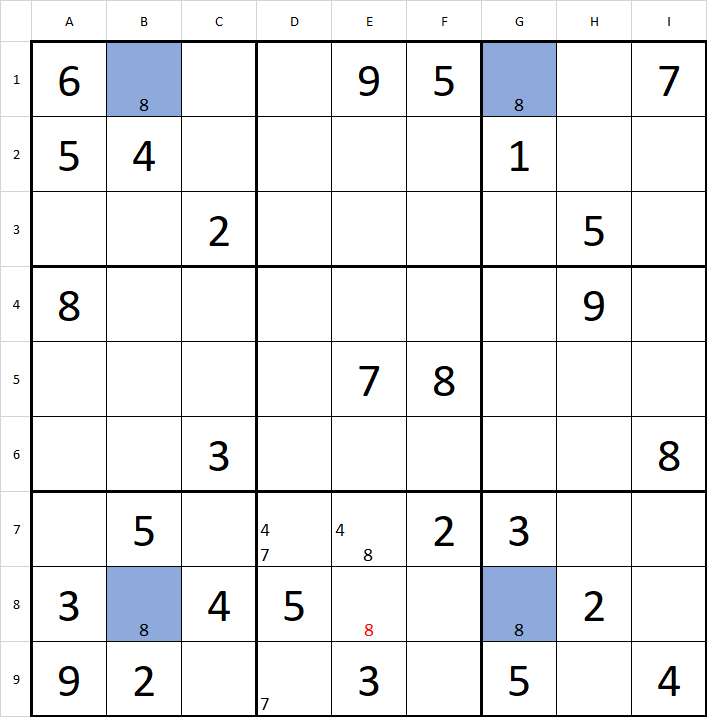
\includegraphics[width=\linewidth]{images/x_wing1.png}
  \caption{Technique removes candidate 8 in E8.}
  \label{fig:xwing1}
\end{subfigure}%
\hfill
\begin{subfigure}[t]{.475\textwidth}
  \centering
  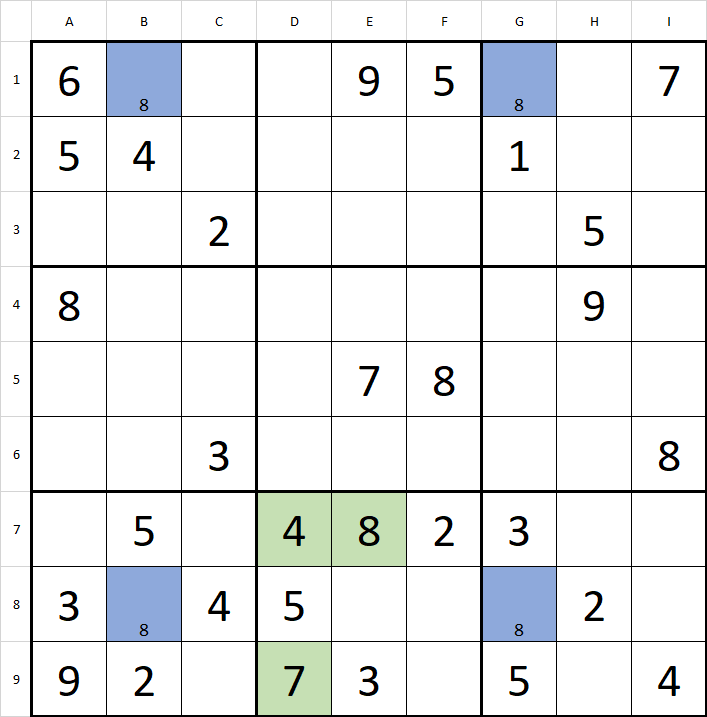
\includegraphics[width=\linewidth]{images/x_wing2.png}
  \caption{Technique led to three filled cells.}
  \label{fig:xwing2}
\end{subfigure}
\caption[X-Wing]{X-Wing highlighted by blue background.}
\label{fig:xwing}
\end{figure}

Due to the restrictions of the game rules, the digits can be only placed diagonally to each other, otherwise the same digit would appear on the same row, or column, which violates the rules. With this information, the player can remove candidates of the same digit in other blocks of the same row, or column \cite{SudokuXW66:online}. In Figure \ref{fig:xwing1} the X-Wing technique is used for the candidate of digit eight, which eventually leads to the removal of one eight and fill out three cells in the 7$^{th}$ block, as seen in Figure \ref{fig:xwing2}.


\subsection{Swordfish}
The Swordfish technique is similar to the \nameref{sec:xwing} technique. A candidate must be in two cells in the same row in three different rows, as seen in Figure \ref{fig:sfish}, which allows to exclude the candidate in the same rows, or columns \cite{SudokuTr32:online}.

\begin{figure}[H]
\centering
\begin{subfigure}[t]{.475\textwidth}
  \centering
  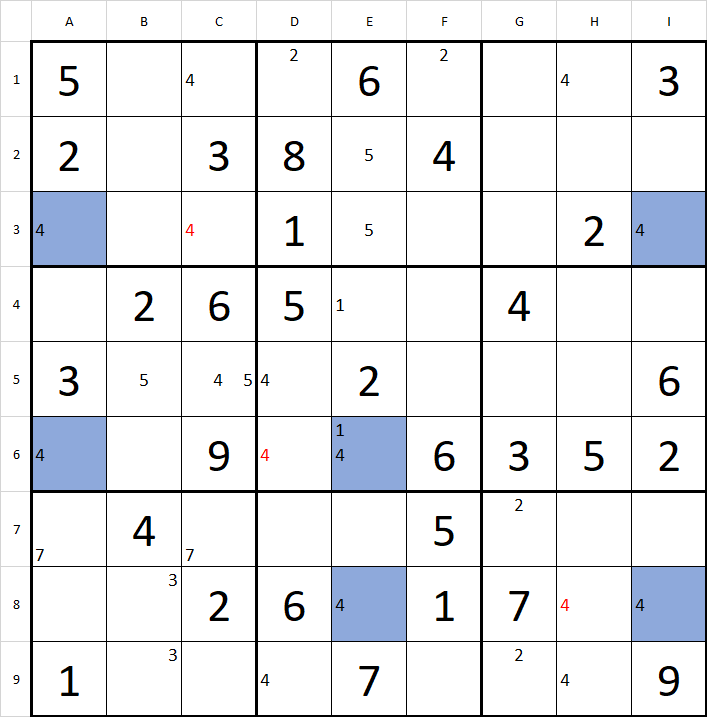
\includegraphics[width=\linewidth]{images/sfish1.png}
  \caption{Candidates for the technique are highlighted with blue background color. Candidates removed by the technique have a red color.}
  \label{fig:sfish1}
\end{subfigure}%
\hfill
\begin{subfigure}[t]{.475\textwidth}
  \centering
  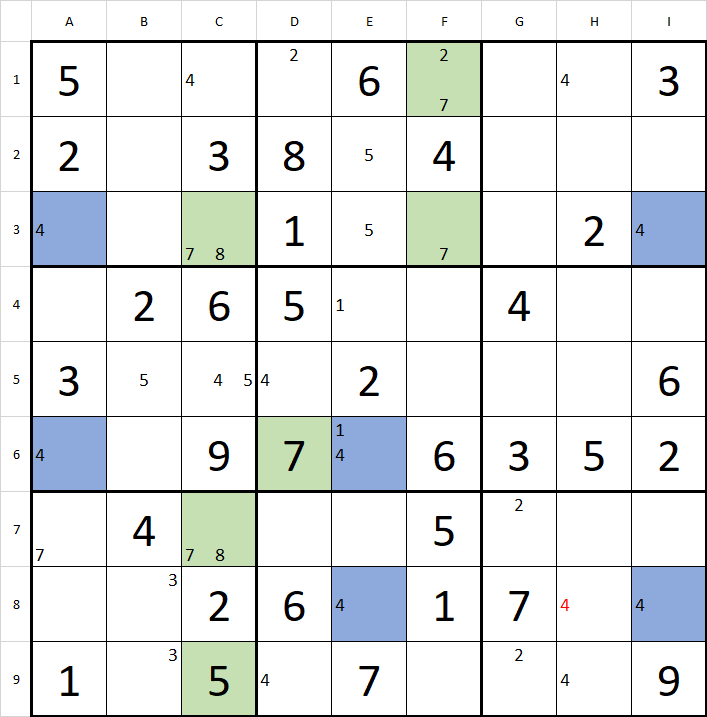
\includegraphics[width=\linewidth]{images/sfish2.png}
  \caption{Due to the removal of candidates, it is possible to put a seven in D6 by using \nameref{ss:lcandidates}, leading to pencil mark the seven in F1 and F3. Additionally, by using \nameref{ss:lcandidates}, it is possible to narrow down three cells: C3 and C7, which forms a \nameref{ss:hpair} and leads to a five in C9.}
  \label{fig:sfish2}
\end{subfigure}

\centering
\begin{subfigure}[t]{.475\textwidth}
  \centering
  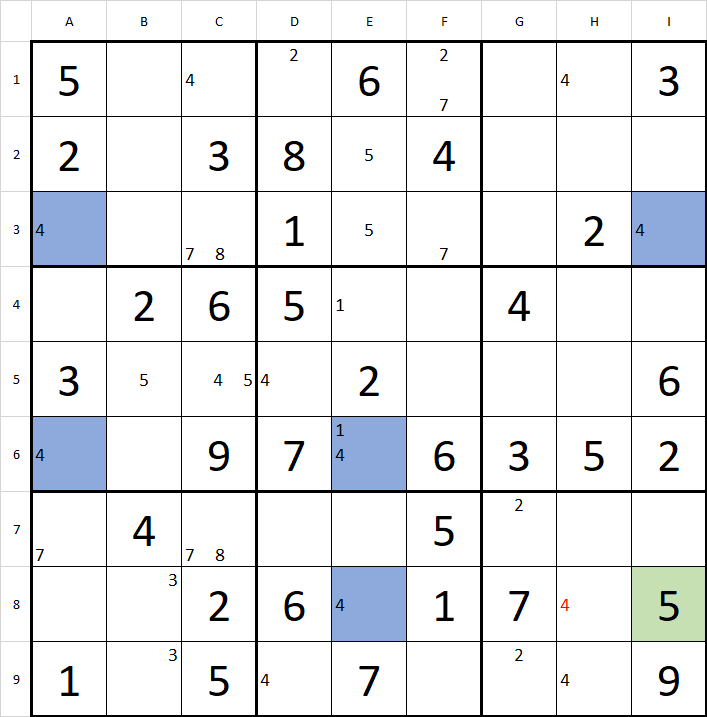
\includegraphics[width=\linewidth]{images/sfish3.png}
  \caption{Due to \nameref{ss:xhatching}, it is possible to place a five in I8.}
  \label{fig:sfish3}
\end{subfigure}%
\hfill
\begin{subfigure}[t]{.475\textwidth}
  \centering
  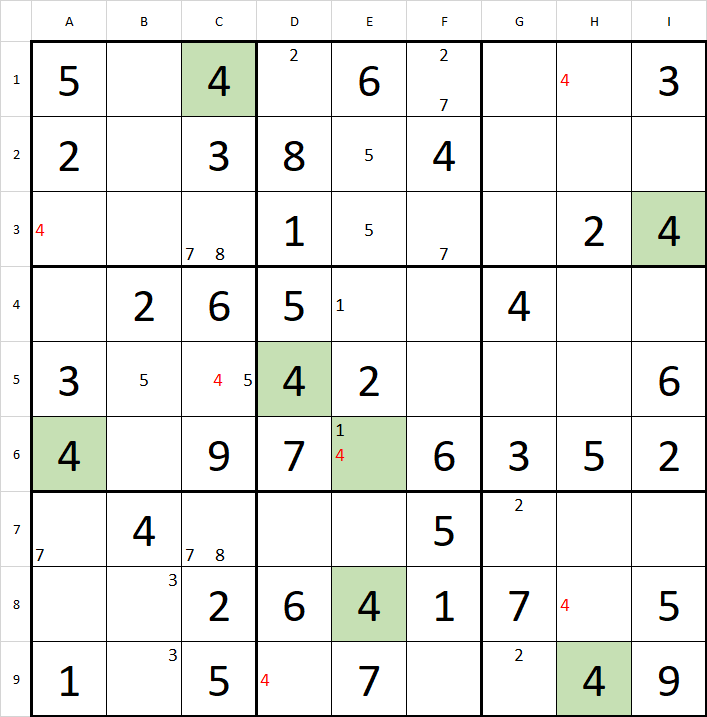
\includegraphics[width=\linewidth]{images/sfish4.png}
  \caption{By placing previously, the five in I8, the candidates for the Swordfish technique got resolved by using \nameref{ss:xhatching}, which led to all fours solved.}
  \label{fig:sfish4}
\end{subfigure}

\caption[Swordfish]{Swordfish demonstration using the \nameref{ss:snydernot}. Source: Adapted from \cite{SudokuTr32:online}}

\label{fig:sfish}
\end{figure}


\subsection{XY-Wing} \label{sec:xywing}
To use the XY-Wing technique, it is required to have three cells with exactly two candidates, which are shared among the three cells in following format: XY (main), YZ (branch), XZ (branch), which is illustrated in Figure \ref{fig:xywing}. Additionally, the main cell must share a group with the branch cells. If these requirements are met, then all cells, which share a group with the branch cells, can eliminate the digit placed for Z \cite{SudokuXY59:online}.

\begin{figure}[H]
  \centering
  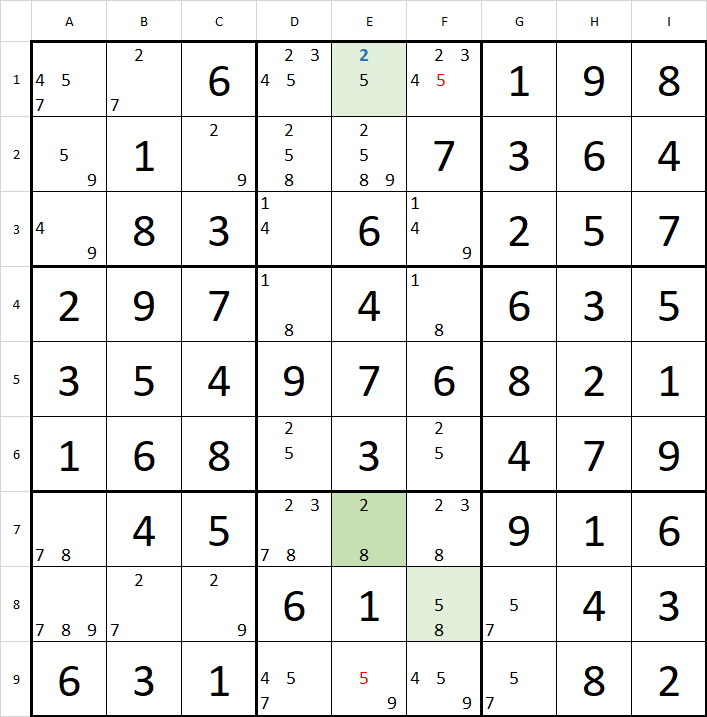
\includegraphics[width=.55\linewidth]{images/xywing}
  \caption[XY-Wing] XY-Wing Technique. The removed candidates are red colored. Main cell highlighted with a green background (E7) and branch cells with light green background (E1, F8). X, Y and Z and represented by 2, 8 and 5, respectively. If E1 takes 2 (X) as its value and F8 takes 8 (Y) as its value, E7 (the main cell) is left out without any candidates. Therefore, the 5 must be in either E1, or F8, which eliminates the candidate in F1 and E9. Source: Adapted from \cite{SolvingS57:online}
  \label{fig:xywing}
\end{figure}%

The logic behind this technique is that if the branch cells would have their respective non-Z digit as their value, it would leave the main cell empty, since both candidates are taken by the branch cells. Therefore, the Z-digit must be in one of the branch cells. 


\subsection{XYZ-Wing}
The XYZ-Wing is an enhanced version of the \nameref{sec:xywing}. In this version, the main branch has also the Z-digit, leading to the elimination of the Z-digit from cells in a group with the main cell. In the XY-Wing technique, it was only a group between the branch cells \cite{XYZWingR68:online}.

\begin{figure}[H]
  \centering
  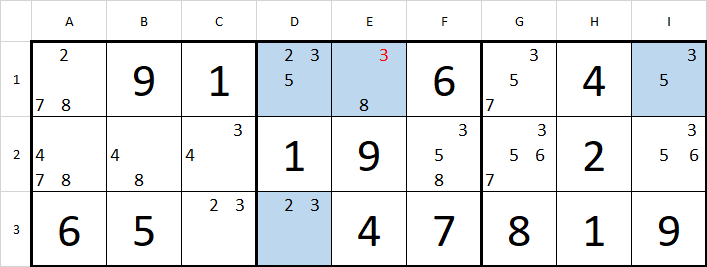
\includegraphics[width=.55\linewidth]{images/xyzwing}
  \caption[XYZ-Wing] XYZ-Wing technique. Affected cells are highlighted with blue background. Main cell is D1, the branch cells are D3 and I1. The red colored digit is the candidate that is eliminated, due to the technique.  Source: Adapted from \cite{XYZWingR68:online}
  \label{fig:xyzwing}
\end{figure}%

Figure \ref{fig:xyzwing} illustrates the effects of this technique. The outcome of the technique is that the candidate with the digit 3 is eliminated in E1, regardless which candidates its value is taken for the main cell in D1.




\chapter{Conclusion}
There are different approaches for solving a puzzle, varying in difficulty. 

The pencil marking techniques have the advantage, that the player does not have to remember every possible candidate for all cells, but can write them down and even use them for further techniques.

The easier techniques, such as Full House and Naked Singles are straight-forward because the player can determine them without much effort. The same applies to Hidden Singles and Naked Pairs, but the player must look closer this time. 

The medium techniques are not as easy to spot because the candidates are "buried" among others, as seen for Hidden Pairs and Locked Candidates. The other two techniques in this category follow a different approach. Previous techniques required the player to only look for candidates in a single block, but the Skyscraper and 2-String kite are different. The player must considerate not only one block, but several with aligning candidates.

The harder techniques require mostly "chained" candidates in varying constellations. This means, that these techniques do not require the candidates to be aligned, but to form a chain with specific candidates. This ensures, that the candidates can be removed from cells, or blocks (depending on the technique), which are not part of the chain. These techniques are harder to spot because it is not necessary, that the candidates have to be aligned and the player might have to look on more than one candidate.

The utilization for these techniques depends on the difficulty of the puzzle. If the puzzle is easy, it is most likely not necessary to use a XYZ-Wing to solve the puzzle. The puzzle can be solved by using much less difficult techniques. Also, it most likely the case that a puzzle can be solved in many ways with different techniques, rather than just one solution. Unless, the puzzle is on expert difficulty, which requires the usage of few, if not single, and hard techniques.








\cleardoublepage
\addcontentsline{toc}{chapter}{References}
\bibliographystyle{apacite} 
\bibliography{sudoku}

















\end{document}